\let\negmedspace\undefined
\let\negthickspace\undefined
\documentclass[report]{IEEEtran}
\usepackage[a5paper, margin=10mm, onecolumn]{geometry}
%\usepackage{lmodern} % Ensure lmodern is loaded for pdflatex
\usepackage{tfrupee} % Include tfrupee package

\setlength{\headheight}{1cm} % Set the height of the header box
\setlength{\headsep}{0mm}     % Set the distance between the header box and the top of the text

\usepackage{gvv-book}
\usepackage{gvv}
\usepackage{cite}
\usepackage{amsmath,amssymb,amsfonts,amsthm}
\usepackage{algorithmic}
\usepackage{graphicx}
\usepackage{textcomp}
\usepackage{xcolor}
\usepackage{txfonts}
\usepackage{listings}
\usepackage{enumitem}
\usepackage{mathtools}
\usepackage{gensymb}
\usepackage{comment}
\usepackage[breaklinks=true]{hyperref}
\usepackage{tkz-euclide} 
\usepackage{listings}
% \usepackage{gvv}                                        
\def\inputGnumericTable{}                                 
\usepackage[latin1]{inputenc}                                
\usepackage{color}                                            
\usepackage{array}                                            
\usepackage{longtable}                                       
\usepackage{calc}                                             
\usepackage{multirow}                                         
\usepackage{hhline}                                           
\usepackage{ifthen}                                           
\usepackage{lscape}
\begin{document}

\bibliographystyle{IEEEtran}
\vspace{3cm}

\title{EE1200 - ELECTRIC CIRCUITS LAB}
\author{EE24BTECH11012 - Bhavanisankar G S \\ EE24BTECH11019 - Dwarak A}
% \maketitle
% \newpage
% \bigskip
{\let\newpage\relax\maketitle}

\renewcommand{\thefigure}{\theenumi}
\renewcommand{\thetable}{\theenumi}
\setlength{\intextsep}{10pt} % Space between text and floats


\numberwithin{equation}{enumi}
\numberwithin{figure}{enumi}
\renewcommand{\thetable}{\theenumi}

\section{How do you capture a one-time event on CRO - show with an example.}

\subsection{AIM : } \\
To capture a one-time event on CRO.

\subsection{APPARATUS REQUIRED : } \\
\begin{itemize}
	\item Oscilloscope
	\item Digital Function generator
	\item A probe
	\item Connecting wires
	\item BNC cables
\end{itemize}

\subsection{Theory : } \\
\begin{itemize}
\item A \color{blue} function generator \color{black} is an electronic device that generates various types of electrical waveforms over a range of frequencies. The most common waveforms produced by a function generator are sine, square, and triangular waves. These waveforms are used to simulate signals in electronic testing and development. The function generator allows the user to adjust the frequency, amplitude, and shape of the waveform, making it a versatile tool in electronics labs.
\item An \color{blue} oscilloscope \color{black} is an electronic test instrument that graphically displays varying signal voltages, usually as a two-dimensional plot of one or more signals as a function of time. The oscilloscope can be used to observe the amplitude, frequency, and shape of the signal waveforms. It captures real-time events by continuously sampling the input signal and displaying it on the screen. Oscilloscopes are essential for diagnosing and troubleshooting electronic circuits, as they provide a visual representation of how signals behave over time.
\item \color{blue} Burst mode \color{black} in a digital function generator refers to a feature that allows the generation of a specific number of cycles of a waveform, followed by a period of no output. This mode is particularly useful for testing circuits that need to respond to a controlled, finite sequence of pulses or cycles.
\item When the \color{blue} SINGLE mode \color{black} is selected, the oscilloscope arms itself to capture a single waveform based on a specified trigger condition. Once the trigger condition is met, the oscilloscope records the waveform and then stops further acquisitions.

\end{itemize}

\subsection{PROCEDURE : } \\
\begin{itemize}
	\item Connect the digital function generator and the oscilloscope using BNC cables and a probe.
	\item Use the function generator in \color{blue} BURST \color{black} mode.
	\item Set the amplitude, frequency and the number of cycles to be captured in the function generator.
	\item Set the mode coupling to normal, run control to single in the oscilloscope and push the manual trigger in the function generator.
	\item A real-time capture of the function input can be seen on the oscilloscope display.
\end{itemize}

\subsection{FIGURES : } \\

\begin{figure}[h]
				 \centering
				 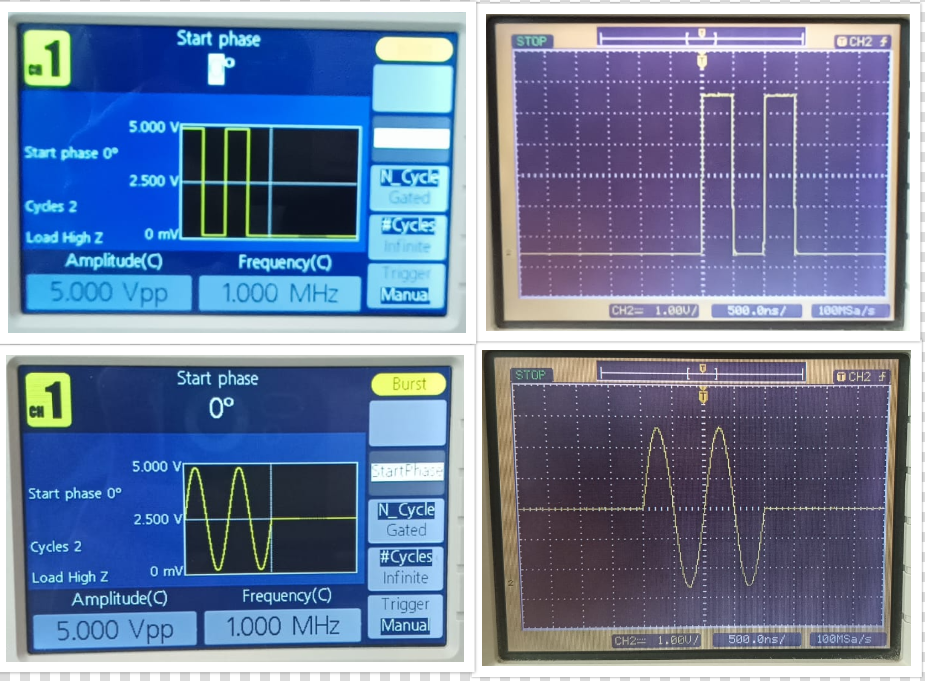
\includegraphics[width=\columnwidth]{fig1.png}
				 \label{fig:Plot1}
			 \end{figure}


\end{document}
